%#!uplatex
\documentclass[a4paper,uplatex]{jsarticle}
\usepackage[driver=dvipdfm,truedimen,margin=2truecm]{geometry}

\usepackage[dvipdfmx]{graphicx}
\usepackage{multirow}

% きれいな枠囲い(必ずgraphicxも有効にし、その後におく)
\usepackage{tcolorbox}

% このページにページ番号を付けたくない時
\thispagestyle{empty}
% 全てのページにページ番号を付けたくない時
%\pagestyle{empty}

\newcommand{\kyou}[1]{{\sffamily\bfseries #1}}

\begin{document}

{\Large 
\begin{center}
電気電子工学実験I 報告書
\vspace*{50mm}

\textsf{\Huge 発振回路の測定}

\vspace*{80mm}

\begin{tabular}{p{40mm}l}
報告者 & E9999 中井 優一\\
共同実験者 & E9998 魚住 花子\\
 & E9997 明石 一郎\\
 & E9996 高専 次郎\\
実験日時 & 2100年1月1日\\
天候 & 晴後曇\\
室温・湿度 & 25度・67\%\\
\end{tabular}
\vspace*{40mm}


 提出期限 2100年2月10日
\end{center}
}


\newpage
\setcounter{page}{1}

\section{目的}

発振回路は信号発生回路とも呼ばれ、ディジタル回路を動作させるためにタ
イミング(同期)をとるクロックパルス信号を発生するだけでなく、AM、FMラジ
オ電波などのさまざまな信号を遠くへ伝えるために使われ、アナログ・ディジ
タルにかかわらずほとんどの電子回路で使用されている。

発振回路は、おおまかに水晶発振回路、セラミック発振回路、CR発振回路、LC
発振回路の4種類がある。水晶発振回路、セラミック発振回路は周波数精度が
非常に高く、発振出力波形にほぼひずみ(誤差)は生じない。一方、CR発振回路、
LC発振回路は周波数精度が水晶発振回路、セラミック発振回路よりも低く、発
信出力波形に十数\%ほどのひずみが生じるが、低価格である。また、CR発振回
路は低周波信号を、LC発振回路は高周波信号を出力するときに用いられる。

\section{ハートレー型LC発振回路}

\subsection{回路図}

図\ref{experiment}にハートレー型LC発振回路の回路図を示す。

\begin{figure}[http]
	\centering
	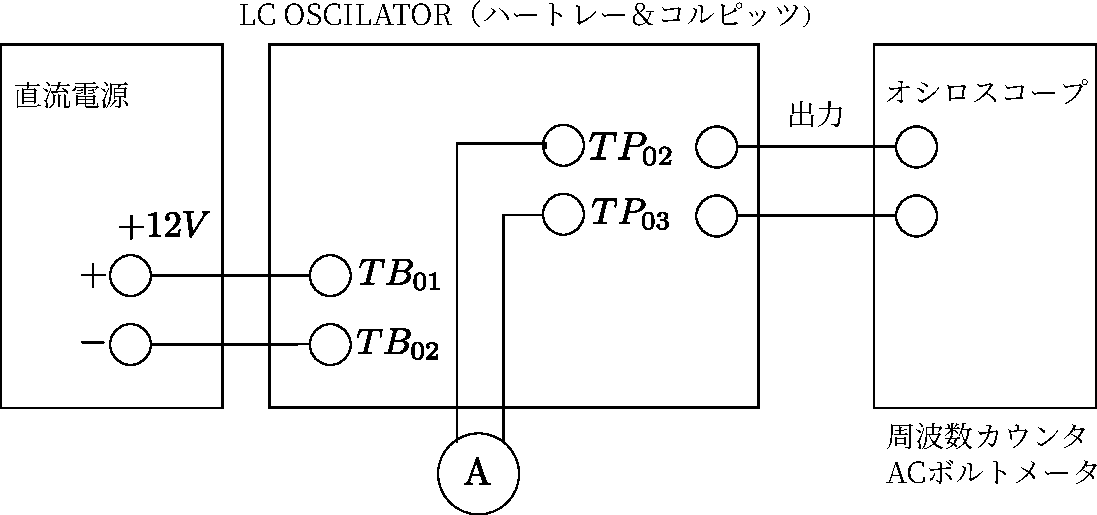
\includegraphics[scale=0.75]{zu.pdf}
	\caption{ハートレー型発振回路の回路図}
	\label{experiment}
\end{figure}


まず、可変コンデンサ$C_{02}$の目盛を0にして出力周波数$f_0$を読むと、
$f_0$=898.61kHzであった。また、ハートレー型の発振周波数の式を式()とし、こ
の式に$f_0$と$C_{02}$を代入して$L_0$を求めた。


実験結果

可変コンデンサ$C_{02}$の目盛を変えた場合の周波数の変化を読み、その時の電圧、
電流も記録した。表にハートレー型LC発振回路の実験結果を示す。
\begin{figure}[http]
	\centering
	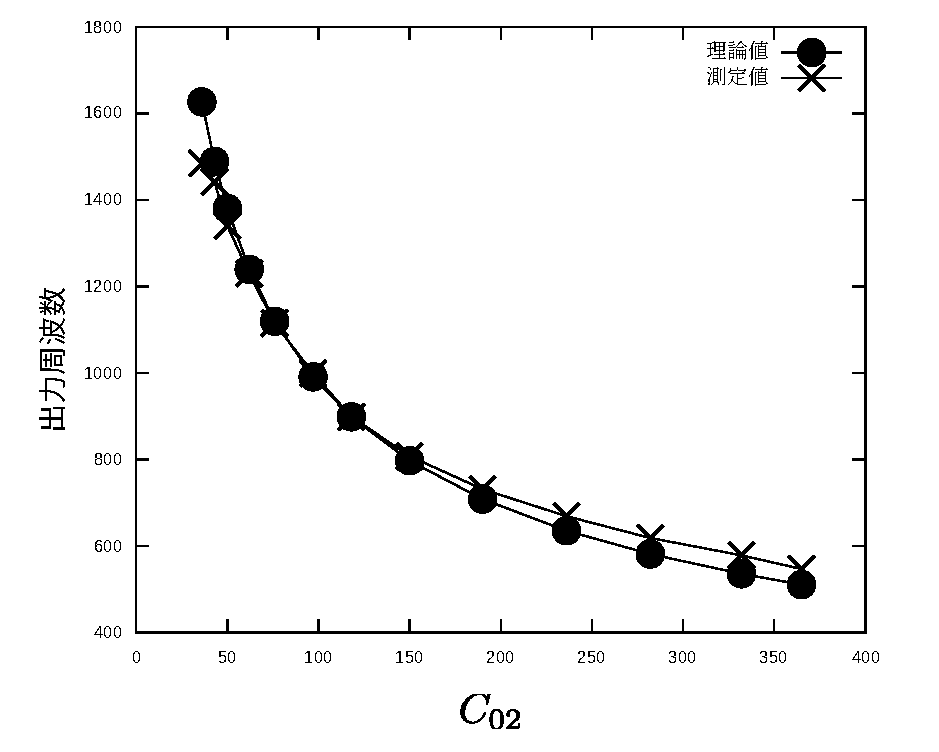
\includegraphics[scale=0.8]{graph.pdf}
	\caption{ハートレー型LC発振回路の実験結果}
	\label{graph}
\end{figure}



表の結果から、図にハートレー型LC発振回路の実験結果のグラフを示す。表と
図からわかるように、$C_{02}$が36pFのときの周波数の理論値、測定値ともに最大と
なっており、$C_{02}$の増加に伴って理論値と測定値は両者の差が小さくなりながら
周波数は反比例のように減少する。周波数が$f_0$=898.6 kHzである$C_{02}$=118pFまで
増加させると、そこを境に測定値が理論値をわずかに上回るということがわかっ
た。また、$C_{02}$が200pFよりも大きくなると、両者はともに周波数の減少する大
きさが小さくなって次第に$C_{02}$の増加に関係なく周波数が一定になることが推測
することができる。

\begin{table}[http]
	\centering
	\caption{ハートレー型LC発振回路の実験結果}
	\label{hartley}
	\begin{tabular}{|r|rr|}
		\hline
		\multicolumn{1}{|c|}{C\_\{02\}}  & \multicolumn{2}{c|}{出力周波数}                                            \\ \hline
		\multicolumn{1}{|l|}{容量{[}pF{]}} & \multicolumn{1}{l|}{理論値{[}kHz{]}} & \multicolumn{1}{l|}{測定値{[}kHz{]}} \\ \hline
		36                               & \multicolumn{1}{r|}{1626.9}       & 1485.0                            \\ \hline
		43                               & \multicolumn{1}{r|}{1488.9}       & 1441.7                            \\ \hline
		50                               & \multicolumn{1}{r|}{1380.5}       & 1340.4                            \\ \hline
		62                               & \multicolumn{1}{r|}{1239.7}       & 1229.9                            \\ \hline
		76                               & \multicolumn{1}{r|}{1119.7}       & 1115.0                            \\ \hline
		97                               & \multicolumn{1}{r|}{991.1}        & 999.1                             \\ \hline
		118                              & \multicolumn{1}{r|}{898.6}        & 898.6                             \\ \hline
		150                              & \multicolumn{1}{r|}{797.0}        & 807.7                             \\ \hline
		190                              & \multicolumn{1}{r|}{708.2}        & 731.4                             \\ \hline
		236                              & \multicolumn{1}{r|}{635.4}        & 668.9                             \\ \hline
		282                              & \multicolumn{1}{r|}{581.3}        & 618.6                             \\ \hline
		332                              & \multicolumn{1}{r|}{535.7}        & 578.4                             \\ \hline
		365                              & \multicolumn{1}{r|}{510.9}        & 546.9                             \\ \hline
	\end{tabular}
\end{table}
次に実験で使用した実験器具を表\ref{tools}に示す。

\begin{table}[]
	\centering
	\caption{実験に使用した器具}
	\label{tools}
	\begin{tabular}{|l|l|l|l|l|}
		\hline
		\multicolumn{1}{|c|}{名称} & \multicolumn{1}{c|}{メーカ} & \multicolumn{1}{c|}{型番} & \multicolumn{1}{c|}{製造番号} & \multicolumn{1}{c|}{管理番号} \\ \hline
		直流電源                     & Metronix                 & 541C                    & 237986                    & B-28-25                   \\ \hline
		オシレータ                    & Yamato Electoronix       & ET-OSI                  &                           &                           \\ \hline
		直流電流計                    & YOKOGAWA                 & 2051                    & 3LU0665                   & は-9-124                   \\ \hline
	\end{tabular}
\end{table}

\section{考察}

\begin{enumerate}
 \item 作成したグラフ(図\ref{graph})について理
       論値と測定値を比較した結果について考察せよ。

       ハートレー型、コルピッツ型で理論値と測定値に誤差が生じる原因につ
       いて、発振周波数が理論値と測定値で等しいことから、直流電源の内部
       抵抗やオシロスコープの内部インピーダンスなどの周辺測定器の影響、
       また、発振器が発生する信号や出力信号に含まれたノイズ成分などの影
       響が重なったからだと考えられる。

       図\ref{graph}の電流の推移において$C_{02}$=118pFを超えると、図\ref{experiment}の$TP_{02}$と$TP_{03}$の2つ
       の端子に接続されたコイルに流れる電流がほぼ一定になった原因につい
       て、$C_{02}$=118pFよりも小さい範囲で周波数が減少するときはコイルのイ
       ンピーダンスが減少するため、コイルに流れる電流が上昇したのだと推
       察する。$C_{02}$=118pFよりも大きい範囲では周波数が一定であるためコイ
       ルのインピーダンスが一定となり、コイルに流れる電流は一定になるの
       だと考えられる。

 \item ハートレー型の周波数特性について考察しどのような用途に適している
       かをのべよ。

       ハートレー型は、図\ref{graph}から$C_{02}$の値の変化に対する周波数の変化が大きかっ
       たことから、AM/FMラジオ受信器に利用されると推測する。ラジオ内部
       にあるハートレー型発振器の$C_{02}$を調節してその番組の周波数と同じ周
       波数に合わせることで共振し、聞きたいラジオ番組を聞くことができる。
\end{enumerate}

\end{document}
